\documentclass[11pt]{article}
\usepackage[margin=1in]{geometry}
\usepackage{enumerate}
\usepackage{framed}
\usepackage{multirow}
\usepackage{multicol}
\usepackage{bm}
\usepackage{amssymb}
\usepackage{amsmath}
\usepackage{amsthm}
\usepackage{multicol}
\usepackage{graphicx}
\setlength{\columnsep}{1in}
\begin{document}

\newcommand{\Name}[1]{\noindent \textbf{Name:} #1 \\}
\newcommand{\pderiv}[2]{\frac{\partial #1}{\partial #2}}
\newcommand{\psderiv}[3]{\frac{\partial^2 #1}{\partial #2 \partial #3}}

\begin{center}
    \bf
    Machine Learning \\
    Computer Science 158 \\
    Spring 2017 \\
    \rm
    Problem Set 7\\
    Due:  March 21 at 11:59 PM \\
\end{center}
\noindent \textbf{Name: Madison Hobbs and Shota Yasunaga} \\

%-------------------- Problem 1 -----------------------%

\section{Feature Extraction [2 pts]}

\begin{enumerate}[(a)]
	\item We implemented \verb+generate_output_codes+.
	\item Below is a plot of the three loss functions $g(z)$ for $z \in [-2, 2]$. 
\begin{center}
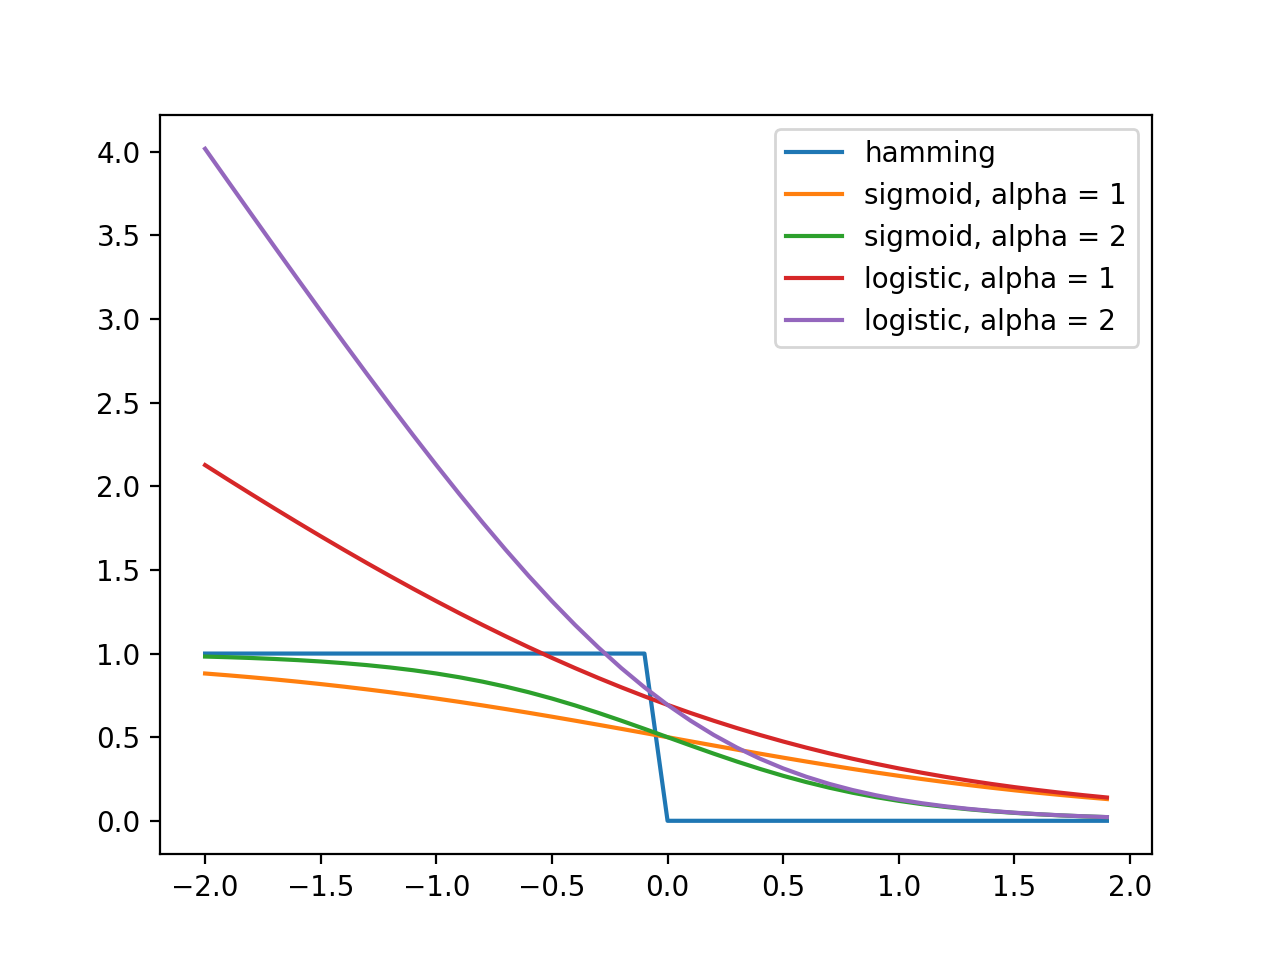
\includegraphics[width = 15cm, height = 10cm]{loss_funcs.png}
\end{center}
	\item We implemented \verb+MulticlassSVM.fit(...)+.
	\item We implemented \verb+MulticlassSVM.predict(...)+.
	\item 
\begin{enumerate}[i.]
	\item Note the following table summarizing our results:
\begin{center}
\begin{tabular}{  c | c | c | c | } 
& hamming loss & sigmoid loss & logistic loss \\
\hline
one versus all & 54 & 46 & 46\\ 
\hline
one versus one & 41 & 48 & 42\\ 
\hline
random (R1) & 38 & 38 & 33\\ 
\hline
random (R2) & 34 & 35 & 34\\ 
\hline
\end{tabular}
\end{center}


	\item For each output code, how do the different loss functions affect the classification results, and why? (You may want to refer back to your plots of the various loss functions.) You do not have to comment on every combination of output code and classifier. Pick the cases that stand out to you, and write a short paragraph (about 5 sentences). \\

	For OVA output code, hamming loss is worst, while sigmoid and logistic losses give equally lower error. Hamming loss says: I don't care much about the magnitude of the error, just whether there's an error or not. However, sigmoid and logisitc loss both penalize more eggregious errors more. The difference between sigmoid and logistic loss is that with logistic loss, we penalize worse errors increasingly more (absolute value of slope increases) whereas with sigmoid loss, we penalize worse errors more but at a decreasing rate (absolute value of slope decreases). We might expect, therefore, for logistic loss to yield a classifier which lets the fewest errors through (lowest error rate). We see that for all the output codes, logistic loss yields as good or better results than the other two loss functions. Only with OVO does hamming loss produce 1 fewer errors than logisitic loss. This could be an artifact of the dataset, and in essense, hamming and logistic losses tie here. It's interesting how hamming loss and logistic loss outperform sigmoid loss in OVO while in all other cases sigmoid and logistic outperform hamming loss (or essentially tie with it). \\

	\item What kind of output code do you think is most suitable for this problem? Why do you think this is the case? Write a short paragraph (about 5 sentences). \\

	Both random output codes yielded the lowest error, so it seems a random output code is most suitable for this problem. Perhaps this is because OVO and OVA are too systematic in checking each class against the other. Maybe the soybean diseases we are predicting are correlated and a lot of the classifiers produced using OVO or OVA are meaningless or fitting to noise. Random output codes may fix this (although it's possible randomness could yield worse classifiers.) Perhaps random output codes homogenize comparisons. 

\end{enumerate}

\end{enumerate}

\section{Digit Recognition using Bagging [5+3 pts]}

In this problem, we will study bagging and random forest on a handwritten digit dataset. This dataset contains 1797 samples (each having 64 features) of hand-written digits, classified into 10 classes.4 However, for this problem, we will only use 720 examples from 4 classes.

\begin{enumerate}[(a)]
	\item \textbf{(3 pts)} Run \verb+main(...)+ to compare the performance of these ensemble classifiers using 100 random splits of the digits dataset into training and test sets, where the test set contains roughly 20\% of the data. This generates two plots : 
We vary the number of features considered for the random forest from 1 to 65 (in step sizes of 2). Then, on a single plot, we plot the accuracy of the bagging classifier against that of the random forest with varying number of features. (Note: This code may take several minutes to run.)

\begin{center}
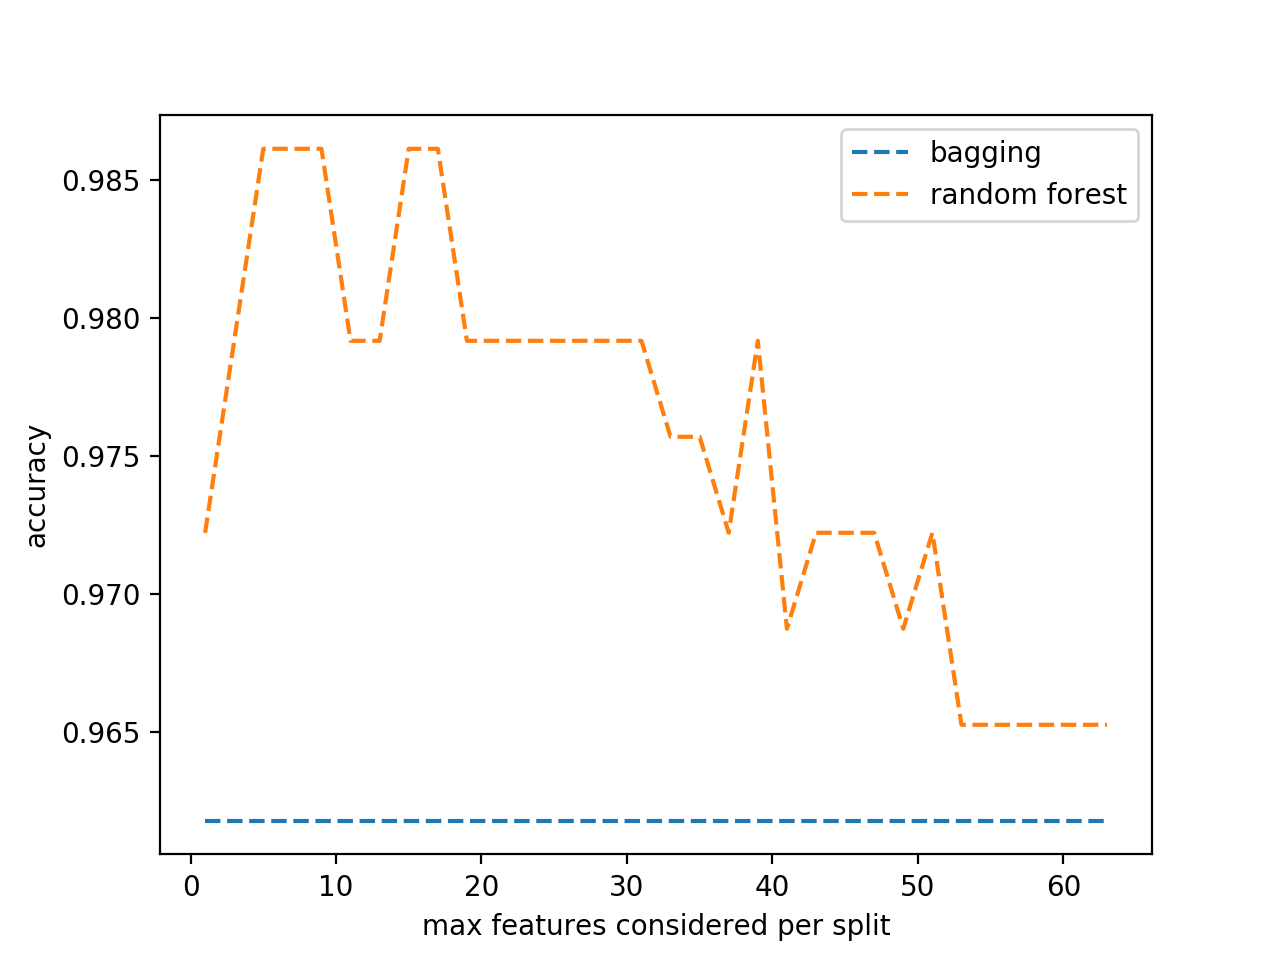
\includegraphics[width = 15cm, height = 10cm]{bag_vs_rf.png}
\end{center}

\begin{center}
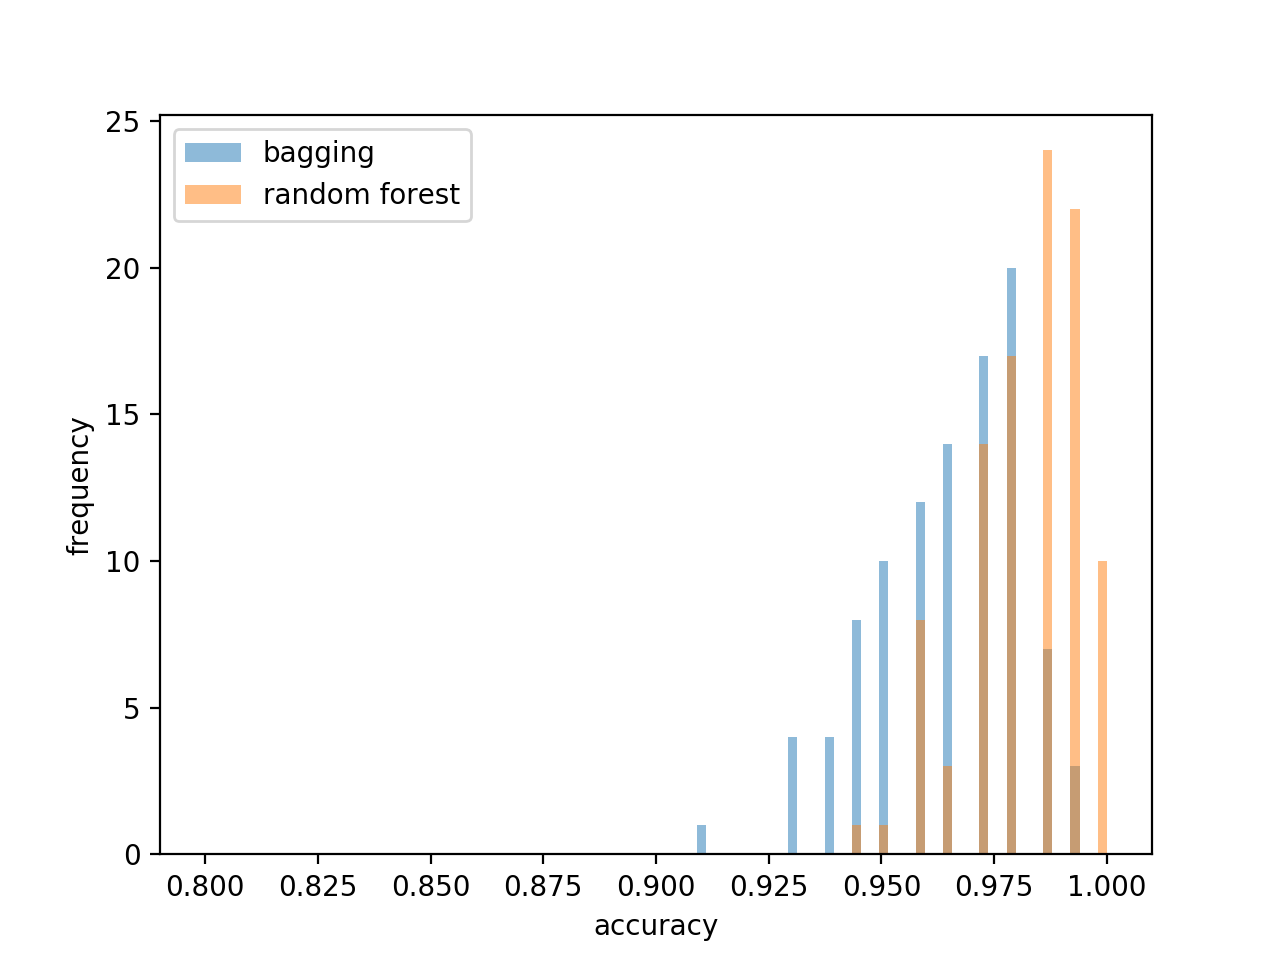
\includegraphics[width = 15cm, height = 10cm]{accuracy.png}
\end{center}
Include these plots in your writeup. How does performance vary with the number of features considered per split? Which classifier performs better, and why?

\textbf{Solution: \\ \\ Random Forest performance varies with the number of features considered at each split, while the bagged trees remains constant. The Random Forest consistently performed better (higher accuracy) than bagged trees. This is probably because the Random Forest has decorrelated trees (each trained using a different subset of features) whereas bagging pulls from the same pool of features in each tree, making them essentially the same/correlated.}

	\item \textbf{(2 pts)} One useful application of bagging ensembles is to assess the relative importance of features. In your own words, describe how you think feature importance might be calculated when using Decision Trees as your base classifier. 

Now, using scikit-learn’s examples as a guideline, generate a representation of the relative importance of each individual pixel for digit recognition (include this plot in your writeup). For this problem, you are allowed to use \verb+sklearn.ensemble.RandomForestClassifier+.

What do you observe? Is this surprising?

\textbf{Solution: \\ We can add up over all the trees how much each feature, when used to make a split, increases information gain. This can measure the importance of that feature by effectively measuring how much it contributes to information gain (how important it is in terms of gaining information about predicting the labels). \\
Below, we see a heat map of the feature importance for this problem. We notice there is just one single pixel in the center that is vastly important, while many pixels (on the periphery) are not that important. It makes sense that pixels on the periphery are not as important (they may not even contain the digit) while pixels towards the center are more important. It is a bit shocking however just how important that one pixel in the center is. 
\begin{center}
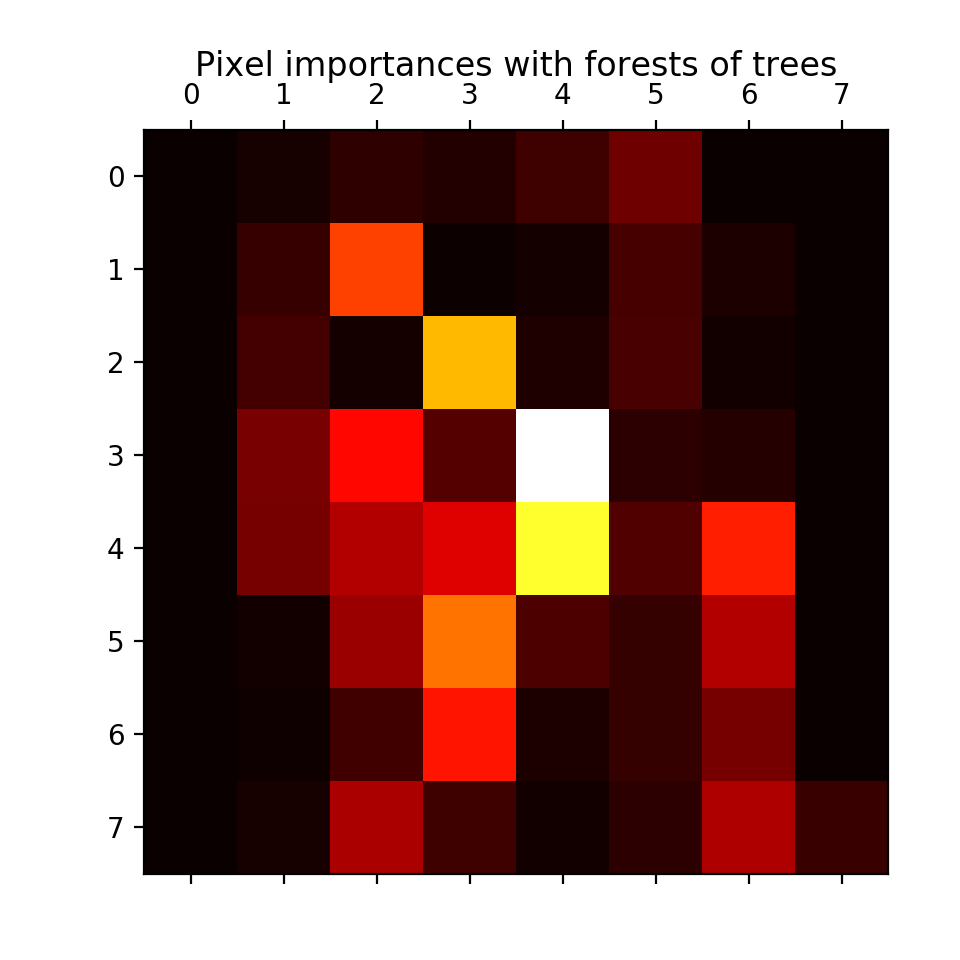
\includegraphics[width = 10cm, height = 10cm]{heatmap.png}
\end{center} }

\end{enumerate}

\end{document}